\section{射影平面上的交比}
%@see: 《解析几何》(丘维声) P269
我们知道,在中心投影下,线段的分比会改变,
但是,射影平面上共线四点的交比保持不变.
我们接下来对这个结论予以证明.

\subsection{交比的定义和性质}
%@see: 《平面解析几何(甲种本)》 P7
%@see: 《解析几何》(丘维声) P269
%@see: 《高等几何(第四版)》(梅向明,刘增贤,王汇淳,王智秋) P1 定义1.1
%@see: 《解析几何》(尤承业) P11
设\(A,B,C\)是欧氏平面\(\pi_0\)上共线三点,\(C \neq B\)(即\(C\)与\(B\)不重合).
如果数\(\lambda\)满足\begin{equation*}
	\vec{AC} = \lambda \vec{CB},
\end{equation*}
则称“\(\lambda\)是点\(C\)分线段\(AB\)所成的\DefineConcept{比}”
“\(\lambda\)是点\(A,B,C\)的\DefineConcept{单比}”
“点\(C\)分线段\(AB\)成定比\(\lambda\)”,
记\(R(A,B,C) \defeq \lambda\),
即\begin{equation*}
%@see: 《解析几何》(丘维声) P269 (3.1)
	R(A,B,C)
	\defeq
	\frac{
		\VectorInnerProductDot{\vec{AC}}{\vec{CB}}
	}{
		\VectorInnerProductDot{\vec{CB}}{\vec{CB}}
	}
	= \frac{\LineSegmentLength{AC}}{\LineSegmentLength{CB}}
	\cos\angle(\vec{AC},\vec{CB})
	\
	\footnote{
		% 《解析几何》(丘维声)、《解析几何》(尤承业)对“共线三点的单比”的定义和正文中的定义相同.
		% 《高等几何(第四版)》(梅向明,刘增贤,王汇淳,王智秋)、《射影几何》(方德植,陈奕培)对“共线三点的单比”的定义和脚注中的定义相同.
		有的书把点\(A,B,C\)的单比\(R(A,B,C)\)定义为\(
			\frac{
				\VectorInnerProductDot{\vec{AC}}{\vec{BC}}
			}{
				\VectorInnerProductDot{\vec{BC}}{\vec{BC}}
			}
		\),
		这样定义的单比与我们在此定义的单比恰好互为相反数.
	}.
\end{equation*}
把点\(A,B\)称为\DefineConcept{基点}.
把点\(C\)称为\DefineConcept{分点}.
这就是过去我们熟知的分点的概念.
根据上述定义,显然不存在点\(C\)使得\(R(A,B,C) = -1\).
因此,我们需要将分点从通常点推广为无穷远点.

设\(A,B,C\)是射影平面\(\overline{\pi_0}\)上共线三点,\(A,B\)是通常点,\(C \neq B\).
当\(C\)是通常点时,规定\(R(A,B,C)\)的定义不变.
当\(C\)是无穷远点时,规定:\begin{equation*}
	R(A,B,C) \defeq -1.
\end{equation*}

\begin{table}[hbt]
	\centering
	\begin{tblr}{c|c}
		\hline
		分点\(C\)相对于线段端点\(A,B\)的位置
		& 分比\(\lambda \defeq R(A,B,C)\) \\
		\hline
		\(C\)在\(AB\)的延长线上
		& \(-\infty<\lambda<-1\) \\
		{\color{red}\(C\)是无穷远点}
		& \(\lambda=-1\) \\
		\(C\)在\(BA\)的延长线上
		& \(-1<\lambda<0\) \\
		\(C\)与\(A\)重合
		& \(\lambda=0\) \\
		\(C\)在\(AB\)的中点与\(A\)之间
		& \(0<\lambda<1\) \\
		\(C\)与\(AB\)的中点重合
		& \(\lambda=1\) \\
		\(C\)在\(AB\)的中点与\(B\)之间
		& \(1<\lambda<+\infty\) \\
		\hline
	\end{tblr}
	\caption{}
\end{table}

\begin{figure}[hbt]
	\centering
	\begin{tikzpicture}
		\begin{axis}[
			xmin=-5,xmax=5,
			ymin=-4,ymax=2,
			grid=none,
			axis lines=middle,
			xlabel=$x$,
			ylabel=$y$,
			enlargelimits,
			enlarge x limits=0.1,
			enlarge y limits=0.1,
			xscale=2,
			xtick={-6,...,6},
			ytick={-4,...,2},
		]
			\addplot[color=blue,samples=20,smooth,domain=-6:0]{x/(1-x)};
			\addplot[color=blue,samples=30,smooth,domain=0:.95]{x/(1-x)};
			\addplot[color=blue,samples=50,smooth,domain=1.05:6]{x/(1-x)};
			\draw[dashed] (1,-6)--(1,-1) (1,0)--(1,4)
				(-6,-1)--(-1,-1) (0,-1)--(6,-1)
				(.5,0)|-(0,1);
			\draw(0,0)coordinate(A)node[above left]{$A$}
				(1,0)coordinate(B)node[above right]{$B$}
				(-3,-3)node{$y=\frac{x}{1-x}$};
		\end{axis}
		\fill(A)circle(2pt) (B)circle(2pt);
	\end{tikzpicture}
	\caption{点$C(x,0)$分线段$AB$所成的比$y=R((0,0),(1,0),(x,0))$}
\end{figure}

\begin{property}
%@see: 《解析几何》(尤承业) P11
设\(A,B,C\)是射影平面\(\overline{\pi_0}\)上共线三点,\(A,B\)是通常点,\(C \neq B\),
则\begin{equation*}
	R(A,B,C) \cdot R(B,A,C) = 1.
\end{equation*}
\begin{proof}
直接计算得\begin{align*}
	R(A,B,C) \cdot R(B,A,C)
	&= \frac{
		\VectorInnerProductDot{\vec{AC}}{\vec{CB}}
	}{
		\VectorInnerProductDot{\vec{CB}}{\vec{CB}}
	}
	\cdot \frac{
		\VectorInnerProductDot{\vec{BC}}{\vec{CA}}
	}{
		\VectorInnerProductDot{\vec{CA}}{\vec{CA}}
	}
	= \frac{
		(\VectorInnerProductDot{\vec{AC}}{\vec{CB}})^2
	}{
		(\VectorInnerProductDot{\vec{CB}}{\vec{CB}})
		(\VectorInnerProductDot{\vec{CA}}{\vec{CA}})
	} \\
	&= \frac{
		\left( \VectorLengthA{\vec{AC}} \VectorLengthA{\vec{AC}} \cos\angle(\vec{AC},\vec{CB}) \right)^2
	}{
		\VectorLengthA{\vec{CB}}^2 \VectorLengthA{\vec{CA}}^2
	}
	= 1.
	\qedhere
\end{align*}
\end{proof}
\end{property}

接下来定义\(\overline{\pi_0}\)上共线四点的交比.
\begin{definition}%\label{definition:解析几何.射影平面上的交比.四点的交比}
%@see: 《解析几何》(丘维声) P269 定义3.1
%@see: 《高等几何(第四版)》(梅向明,刘增贤,王汇淳,王智秋) P29 定义1.1
设\(A,B,C,D\)是射影平面\(\overline{\pi_0}\)上共线四点,
\(A,B\)是通常点,
\(
	A \neq B,
	C \neq B,
	D \neq A
\).
定义:\begin{equation*}
%@see: 《解析几何》(丘维声) P270 (3.2)
%@see: 《高等几何(第四版)》(梅向明,刘增贤,王汇淳,王智秋) P29 (1.1)
	R(A,B,C,D)
	\defeq
	\begin{cases}[cl]
		\frac{R(A,B,C)}{R(A,B,D)},	& D \neq B, \\
		0,							& D = B.
	\end{cases}
\end{equation*}
称之为“点\(A,B,C,D\)的\DefineConcept{交比}”
“点\(A,B,C,D\)的\DefineConcept{复比}”
“点\(A,B,C,D\)的\DefineConcept{二重比}”.
把点\(A,B\)称为\DefineConcept{基点偶}.
把点\(C,D\)称为\DefineConcept{分点偶}.
\end{definition}

\begin{property}
%@see: 《高等几何(第四版)》(梅向明,刘增贤,王汇淳,王智秋) P29
设\(A,B,C,D\)是射影平面\(\overline{\pi_0}\)上共线四点,
\(A,B\)是通常点,
\(
	A \neq B,
	C \neq B,
	D \neq A
\).
\begin{itemize}
	\item 当分点偶\(C,D\)不分离基点偶\(A,B\)
	(如\cref{figure:解析几何.射影平面上的交比.四点的交比大于零1,figure:解析几何.射影平面上的交比.四点的交比大于零2} 所示)时,
	有\begin{equation*}
		R(A,B,C,D) > 0.
	\end{equation*}

	\item 当分点偶\(C,D\)分离基点偶\(A,B\)
	(如\cref{figure:解析几何.射影平面上的交比.四点的交比小于零1,figure:解析几何.射影平面上的交比.四点的交比小于零2} 所示)时,
	有\begin{equation*}
		R(A,B,C,D) < 0.
	\end{equation*}

	\item 当\(C\)与\(D\)重合时,有\begin{equation*}
		R(A,B,C,D) = 1.
	\end{equation*}

	\item 当\(C\)与\(A\)重合时,有\begin{equation*}
		R(A,B,C,D) = 0.
	\end{equation*}
\end{itemize}
\end{property}
\begin{figure}[hbt]
%@see: 《高等几何(第四版)》(梅向明,刘增贤,王汇淳,王智秋) P29 图3-1
%@see: 《高等几何(第四版)》(梅向明,刘增贤,王汇淳,王智秋) P29 图3-2
	\centering
	\def\subwidth{.4\linewidth}
	\begin{subfigure}[b]{\subwidth}
		\centering
		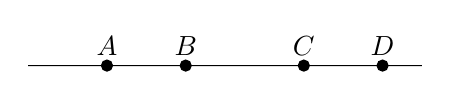
\begin{tikzpicture}
			\filldraw(0,0)--(5,0)
				(1,0)circle(2pt)node[above]{$A$}
				(2,0)circle(2pt)node[above]{$B$}
				(3.5,0)circle(2pt)node[above]{$C$}
				(4.5,0)circle(2pt)node[above]{$D$};
		\end{tikzpicture}
		\caption{}
		\label{figure:解析几何.射影平面上的交比.四点的交比大于零1}
	\end{subfigure}~\begin{subfigure}[b]{\subwidth}
		\centering
		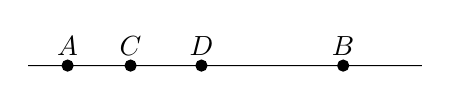
\begin{tikzpicture}
			\filldraw(0,0)--(5,0)
				(.5,0)circle(2pt)node[above]{$A$}
				(1.3,0)circle(2pt)node[above]{$C$}
				(2.2,0)circle(2pt)node[above]{$D$}
				(4,0)circle(2pt)node[above]{$B$};
		\end{tikzpicture}
		\caption{}
		\label{figure:解析几何.射影平面上的交比.四点的交比大于零2}
	\end{subfigure}
	\begin{subfigure}[b]{\subwidth}
		\centering
		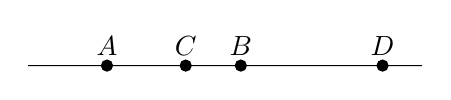
\begin{tikzpicture}
			\filldraw(0,0)--(5,0)
				(1,0)circle(2pt)node[above]{$A$}
				(2,0)circle(2pt)node[above]{$C$}
				(2.7,0)circle(2pt)node[above]{$B$}
				(4.5,0)circle(2pt)node[above]{$D$};
		\end{tikzpicture}
		\caption{}
		\label{figure:解析几何.射影平面上的交比.四点的交比小于零1}
	\end{subfigure}~\begin{subfigure}[b]{\subwidth}
		\centering
		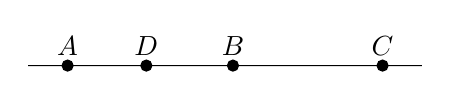
\begin{tikzpicture}
			\filldraw(0,0)--(5,0)
				(.5,0)circle(2pt)node[above]{$A$}
				(1.5,0)circle(2pt)node[above]{$D$}
				(2.6,0)circle(2pt)node[above]{$B$}
				(4.5,0)circle(2pt)node[above]{$C$};
		\end{tikzpicture}
		\caption{}
		\label{figure:解析几何.射影平面上的交比.四点的交比小于零2}
	\end{subfigure}
	\caption{}
\end{figure}

类似地,我们也可以给射影平面上共点四线规定它们的交比.
\begin{definition}\label{definition:解析几何.射影平面上的交比.四线的交比}
设\(\AutoTuple{l}{4}\)是射影平面\(\overline{\pi_0}\)上经过点\(O\)的四条直线,
\(l_1 \neq l_2\).
任取一条不经过点\(O\)的直线\(l\),
与\(\AutoTuple{l}{4}\)分别交于\(\AutoTuple{A}{4}\).
如果\(R(\AutoTuple{A}{4})\)有定义,
则将点\(\AutoTuple{A}{4}\)的交比\(R(\AutoTuple{A}{4})\)
称为“直线\(\AutoTuple{l}{4}\)的\DefineConcept{交比}”,
记作\(R(\AutoTuple{l}{4})\),
即\begin{equation*}
%@see: 《解析几何》(丘维声) P270 (3.3)
	R(\AutoTuple{l}{4})
	\defeq
	R(\AutoTuple{A}{4}).
\end{equation*}
\end{definition}

下面来证明\cref{definition:解析几何.射影平面上的交比.四线的交比} 是有意义的,
即这样定义的交比与直线\(l\)(称为\DefineConcept{截线})的选取无关.
为此,在\(\pi_0\)上取定一个仿射标架\([O;\AutoTuple{d}{2}]\),
设直线\(l_i\)的齐次坐标为\((\eta_{i1},\eta_{i2},\eta_{i3})\),
点\(A_i\)的齐次坐标为\((a_{i1},a_{i2},a_{i3})\ (i=1,2,3,4)\).
因为\(l_1 \neq l_2\),
由\hyperref[example:解析几何.射影平面上的对偶原理.三线共点的条件]{三线共点的条件}可知\begin{equation*}
	% \eta_{3j} = \lambda_1 \eta_{1j} + \mu_1 \eta_{2j},
	% \qquad
	% \eta_{4j} = \lambda_2 \eta_{1j} + \mu_2 \eta_{2j}
	% \quad(j=1,2,3).
	\begin{bmatrix}
		\eta_{31} \\
		\eta_{32} \\
		\eta_{33}
	\end{bmatrix}
	= \lambda_1
	\begin{bmatrix}
		\eta_{11} \\
		\eta_{12} \\
		\eta_{13}
	\end{bmatrix}
	+ \mu_1
	\begin{bmatrix}
		\eta_{21} \\
		\eta_{22} \\
		\eta_{23}
	\end{bmatrix},
	\qquad
	\begin{bmatrix}
		\eta_{41} \\
		\eta_{42} \\
		\eta_{43}
	\end{bmatrix}
	= \lambda_2
	\begin{bmatrix}
		\eta_{11} \\
		\eta_{12} \\
		\eta_{13}
	\end{bmatrix}
	+ \mu_2
	\begin{bmatrix}
		\eta_{21} \\
		\eta_{22} \\
		\eta_{23}
	\end{bmatrix},
\end{equation*}
即\begin{equation*}
	\begin{bmatrix}
		\eta_{31} & \eta_{41} \\
		\eta_{32} & \eta_{42} \\
		\eta_{33} & \eta_{43}
	\end{bmatrix}
	= \begin{bmatrix}
		\eta_{11} & \eta_{21} \\
		\eta_{12} & \eta_{22} \\
		\eta_{13} & \eta_{23}
	\end{bmatrix}
	\begin{bmatrix}
		\lambda_1 & \lambda_2 \\
		\mu_1 & \mu_2
	\end{bmatrix}.
\end{equation*}
在仿射坐标系中,
若点\(M_1(x_1,y_1)\)与\(M_2(x_2,y_2)\)的连线
与直线\(A x + B y + C = 0\)的交点为\(M\),
则\begin{equation*}
%@Mathematica: sol = Solve[{(x - x1)/(x2 - x1) == (y - y1)/(y2 - y1), a x + b y + c == 0}, {x, y}]
%@Mathematica: M1 = {x1, y1};
%@Mathematica: M2 = {x2, y2};
%@Mathematica: M = {x, y};
%@Mathematica: M1M = M - M1;
%@Mathematica: MM2 = M2 - M;
%@Mathematica: R = M1M.MM2/MM2.MM2;
%@Mathematica: R /. sol[[1]] // FullSimplify
	R(M_1,M_2,M)
	= -\frac{A x_1 + B y_1 + C}{A x_2 + B y_2 + C}.
\end{equation*}
因此,我们得到\begin{equation*}
	R(A_1,A_2,A_3)
	= -\frac{\eta_{31} \dfrac{a_{11}}{a_{13}} + \eta_{32} \dfrac{a_{12}}{a_{13}} + \eta_{33}}
			{\eta_{31} \dfrac{a_{21}}{a_{23}} + \eta_{32} \dfrac{a_{22}}{a_{23}} + \eta_{33}}
	= -\frac{\mu_1 \left( \eta_{21} \dfrac{a_{11}}{a_{13}} + \eta_{22} \dfrac{a_{12}}{a_{13}} + \eta_{23} \right)}
			{\lambda_1 \left( \eta_{11} \dfrac{a_{12}}{a_{23}} + \eta_{12} \dfrac{a_{22}}{a_{23}} + \eta_{13} \right)},
\end{equation*}
同理可得\begin{equation*}
	R(A_1,A_2,A_4)
	= -\frac{\mu_2 \left( \eta_{21} \dfrac{a_{11}}{a_{13}} + \eta_{22} \dfrac{a_{12}}{a_{13}} + \eta_{23} \right)}
			{\lambda_2 \left( \eta_{11} \dfrac{a_{21}}{a_{23}} + \eta_{12} \dfrac{a_{22}}{a_{23}} + \eta_{13} \right)}.
\end{equation*}
于是\begin{equation}\label{equation:解析几何.射影平面上的交比.四线的交比1}
%@see: 《解析几何》(丘维声) P271 (3.4)
	R(l_1,l_2,l_3,l_4)
	= R(A_1,A_2,A_3,A_4)
	= \frac{\mu_1 \lambda_2}{\lambda_1 \mu_2}
	= \frac{\lambda_2}{\mu_2} \bigg/ \frac{\lambda_1}{\mu_1}.
\end{equation}
由此可见,\cref{definition:解析几何.射影平面上的交比.四线的交比} 中
共线四点的交比只与这四条直线的相互位置有关,而与截线\(l\)的选取无关.

\begin{figure}[hbt]
%@see: 《解析几何》(丘维声) P271 图7.8
	\centering
	\begin{tikzpicture}[
		label distance=2pt,
	]
		% 依赖 tkz-euclide 宏包
		\coordinate[label=right:$O$](O)at(0,0);
		\coordinate[label=above left:$A_1$](A1)at(-3,-3);
		\coordinate[label=above left:$A_2$](A2)at(-1,-3);
		\coordinate[label=above left:$A_3$](A3)at(1,-3);
		\coordinate[label=above right:$A_4$](A4)at(2,-3);

		\coordinate[label=above left:$A_1'$](A1')at($(O)!.6!(A1)$);
		\coordinate[label=above left:$A_2'$](A2')at($(O)!.55!(A2)$);
		\coordinate[label=above left:$A_3'$](A3')at($(O)!.5!(A3)$);
		\coordinate[label=above right:$A_4'$](A4')at($(O)!.45!(A4)$);

		\tkzDrawLines(A1,A4 O,A1 O,A2 O,A3 O,A4)
		\tkzDrawLine[add=.2 and .6](A1',A4')

		\draw($(A3)!2!(A4)$)node[above]{$l$};
		\draw($(A3')!4.5!(A4')$)node[right]{$l'$};
		\draw($(A1')!1.2!(A1)$)node[below right]{$l_1$};
		\draw($(A2')!1.2!(A2)$)node[below right]{$l_2$};
		\draw($(A3')!1.2!(A3)$)node[below left]{$l_3$};
		\draw($(A4')!1.2!(A4)$)node[below left]{$l_4$};
	\end{tikzpicture}
	\caption{}
	\label{figure:解析几何.射影平面上的交比.四线的交比1}
\end{figure}

如\cref{figure:解析几何.射影平面上的交比.四线的交比1} 所示,
在以\(O\)为中心的中心投影下,
设\(l\)的像为\(l'\),
\(l'\)与\(l_i\)的交点为\(A_i'\ (i=1,2,3,4)\),
则在这个中心投影下,
\(A_i\)的像是\(A_i'\ (i=1,2,3,4)\).
根据上面的讨论,共点四线的交比与截线的选取无关,得\begin{equation*}
	R(A_1,A_2,A_3,A_4)
	= R(l_1,l_2,l_3,l_4)
	= R(A_1',A_2',A_3',A_4').
\end{equation*}
因此在中心投影下交比保持不变.

由于中心投影可以分解成射影和截影两个步骤,
因此交比在射影和截影下保持不变.
据此可以推广前述交比的定义,
免除前面定义交比时所加上的某些元素不能是无穷远元素的限制.
给定共线四点\(A,B,C,D\),
若\(A,B,C\)各不相同,
并且\(D \neq A\),
则可以把它们的交比\(R(A,B,C,D)\)规定为
它们在某个点\(O\)上的射影\(OA,OB,OC,OD\)的交比;
给定共点四线\(l_1,l_2,l_3,l_4\),
若\(l_1,l_2,l_3\)各不相同,
并且\(l_4 \neq l_1\),
则可以把它们的交比\(R(l_1,l_2,l_3,l_4)\)规定为
它们在某条直线\(l\)上的截影\(P_1,P_2,P_3,P_4\)的交比.
这样规定的交比仍然包含前面的定义作为特例,并且具有性质:
交比在上述射影和截影下保持不变.
这样一来,我们在讨论交比的性质时,
总可以假设它们是共线的四个通常点的交比,
因为如果共线的四个点中有无穷远点,
我们总可以经过射影和截影,把它们变成共线的四个通常点.
如\cref{figure:解析几何.射影平面上的交比.四线的交比2} 所示,
点\(A_1\)是无穷远点,
但是它在点\(O\)上的射影\(OA_1\)在直线\(l'\)上的截影\(A_1'\)是一个通常点.

\begin{figure}[hbt]
%@see: 《解析几何》(丘维声) P272 图7.9
	\centering
	\begin{tikzpicture}[
		label distance=2pt,
	]
		% 依赖 tkz-euclide 宏包
		\coordinate[label=above right:$O$](O)at(0,0);
		\coordinate[label=above left:$A_1$](A1)at(-3,0);
		\coordinate[label=above left:$A_2$](A2)at(-1,-3);
		\coordinate[label=above left:$A_3$](A3)at(1,-3);
		\coordinate[label=above left:$A_4$](A4)at(2,-3);

		\coordinate[label=above right:$A_1'$](A1')at($(O)!.6!(A1)$);
		\coordinate[label=above right:$A_4'$](A4')at($(O)!.45!(A4)$);

		\tkzDrawLines(A2,A4 A1',A4' O,A1 O,A2 O,A3 O,A4)
		\tkzInterLL(A1',A4')(O,A2) \tkzGetPoint{A2'}
		\tkzInterLL(A1',A4')(O,A3) \tkzGetPoint{A3'}

		\draw(A2')+(200:15pt)node[]{$A_2'$};
		\draw(A3')node[below left]{$A_3'$};

		\draw($(A3)!2!(A4)$)node[above]{$l$};
		\draw($(A1')!1.2!(A4')$)node[right]{$l'$};
	\end{tikzpicture}
	\caption{}
	\label{figure:解析几何.射影平面上的交比.四线的交比2}
\end{figure}

我们已经会用直线的齐次坐标计算共点四线的交比,现在我们来讨论如何用点的齐次坐标计算共线四点的交比.
\begin{theorem}%\label{theorem:解析几何.射影平面上的交比.四点的交比1}
%@see: 《解析几何》(丘维声) P272 定理3.1
设\(A,B,C,D\)是射影平面\(\overline{\pi_0}\)上共线四点,
其中\(A,B,C\)各不相同,
并且\(D \neq A\),
又设\(A,B,C,D\)的齐次坐标分别为\(
	(\AutoTuple{a}{3}),
	(\AutoTuple{b}{3}),
	(\AutoTuple{c}{3}),
	(\AutoTuple{d}{3})
\),
且\begin{equation*}
	\begin{bmatrix}
		c_1 & d_1 \\
		c_2 & d_2 \\
		c_3 & d_3
	\end{bmatrix}
	= \begin{bmatrix}
		a_1 & b_1 \\
		a_2 & b_2 \\
		a_3 & b_3
	\end{bmatrix}
	\begin{bmatrix}
		\lambda_1 & \lambda_2 \\
		\mu_1 & \mu_2
	\end{bmatrix},
\end{equation*}
则\begin{equation*}\label{equation:解析几何.射影平面上的交比.四点的交比1}
%@see: 《解析几何》(丘维声) P272 (3.5)
	R(A,B,C,D)
	= \frac{\lambda_2}{\mu_2} \bigg/ \frac{\lambda_1}{\mu_1}.
\end{equation*}
\end{theorem}

共线四点的交比还可以通过另一种形式来计算.
\begin{theorem}\label{theorem:解析几何.射影平面上的交比.四点的交比2}
%@see: 《解析几何》(丘维声) P273 定理3.2
设\(A,B,C,D\)是射影平面\(\overline{\pi_0}\)上共线四点,
其中\(A,B,C\)各不相同,
并且\(D \neq A\).
在直线\(ABCD\)上取两点\(P,Q\),
设它们的齐次坐标分别为\(
	(\AutoTuple{p}{3}),
	(\AutoTuple{q}{3})
\),
又设\(A,B,C,D\)的齐次坐标分别为\(
	(\AutoTuple{a}{3}),
	(\AutoTuple{b}{3}),
	(\AutoTuple{c}{3}),
	(\AutoTuple{d}{3})
\),
且\begin{equation*}
	\begin{bmatrix}
		a_1 & b_1 & c_1 & d_1 \\
		a_2 & b_2 & c_2 & d_2 \\
		a_3 & b_3 & c_3 & d_3
	\end{bmatrix}
	= \begin{bmatrix}
		p_1 & q_1 \\
		p_2 & q_2 \\
		p_3 & q_3
	\end{bmatrix}
	\begin{bmatrix}
		\lambda_1 & \lambda_2 & \lambda_3 & \lambda_4 \\
		\mu_1 & \mu_2 & \mu_3 & \mu_4
	\end{bmatrix},
\end{equation*}
则\begin{equation*}\label{equation:解析几何.射影平面上的交比.四点的交比2}
%@see: 《解析几何》(丘维声) P273 (3.6)
	R(A,B,C,D)
	= \frac{
		\begin{vmatrix}
			\lambda_1 & \lambda_3 \\
			\mu_1 & \mu_3
		\end{vmatrix}
		\begin{vmatrix}
			\lambda_2 & \lambda_4 \\
			\mu_2 & \mu_4
		\end{vmatrix}
	}{
		\begin{vmatrix}
			\lambda_1 & \lambda_4 \\
			\mu_1 & \mu_4
		\end{vmatrix}
		\begin{vmatrix}
			\lambda_2 & \lambda_3 \\
			\mu_2 & \mu_3
		\end{vmatrix}
	}.
\end{equation*}
\end{theorem}

从\cref{theorem:解析几何.射影平面上的交比.四点的交比2} 不难得出交比具有下列性质.
\begin{property}
%@see: 《解析几何》(丘维声) P274
%@see: 《高等几何(第四版)》(梅向明,刘增贤,王汇淳,王智秋) P30 定理1.1
设\(A,B,C,D\)是射影平面\(\overline{\pi_0}\)上共线四点,
其中\(A,B,C\)各不相同,
并且\(D \neq A\),
则\begin{equation*}
%@see: 《高等几何(第四版)》(梅向明,刘增贤,王汇淳,王智秋) P30 (1.3)
	R(C,D,A,B)
	= R(A,B,C,D).
\end{equation*}
\end{property}
\begin{remark}
上述性质说明:基点偶与分点偶交换时,交比不变.
\end{remark}

\begin{property}
%@see: 《解析几何》(丘维声) P274
%@see: 《高等几何(第四版)》(梅向明,刘增贤,王汇淳,王智秋) P30 定理1.2
设\(A,B,C,D\)是射影平面\(\overline{\pi_0}\)上共线四点,
其中\(A,B,C\)各不相同,
并且\(D \neq A\),\(D \neq B\),
则\begin{equation*}
%@see: 《高等几何(第四版)》(梅向明,刘增贤,王汇淳,王智秋) P30 (1.4)
	R(B,A,C,D)
	= \frac1{R(A,B,C,D)}
	= R(A,B,D,C).
\end{equation*}
\end{property}
\begin{remark}
上述性质说明:基点偶对换或分点偶对换时,交比变为原交比的倒数.
\end{remark}

\begin{property}
%@see: 《解析几何》(丘维声) P274
%@see: 《高等几何(第四版)》(梅向明,刘增贤,王汇淳,王智秋) P30 推论
设\(A,B,C,D\)是射影平面\(\overline{\pi_0}\)上共线四点,
其中\(A,B,C\)各不相同,
并且\(D \neq A\),
则\begin{equation*}
%@see: 《高等几何(第四版)》(梅向明,刘增贤,王汇淳,王智秋) P30 (1.5)
	R(B,A,D,C)
	= R(A,B,C,D).
\end{equation*}
\end{property}
\begin{remark}
上述性质说明:基点偶、分点偶同时对换时,交比不变.
\end{remark}

\begin{property}
%@see: 《解析几何》(丘维声) P274
%@see: 《高等几何(第四版)》(梅向明,刘增贤,王汇淳,王智秋) P30 定理1.3
设\(A,B,C,D\)是射影平面\(\overline{\pi_0}\)上共线四点,
其中\(A,B,C\)各不相同,
并且\(D \neq A\),
则\begin{equation*}
%@see: 《高等几何(第四版)》(梅向明,刘增贤,王汇淳,王智秋) P30 (1.6)
	R(A,C,B,D)
	= R(D,B,C,A)
	= 1 - R(A,B,C,D).
\end{equation*}
\end{property}

由对偶原理可知,对于共点四线的交比,
也有类似于\cref{theorem:解析几何.射影平面上的交比.四点的交比2} 的计算公式和上述三条性质.

共点四线还有一条重要性质.
\begin{property}
%@see: 《解析几何》(丘维声) P274
%@see: 《解析几何》(丘维声) P277 习题7.3 8.
设\(\AutoTuple{l}{4}\)是射影平面\(\overline{\pi_0}\)上经过通常点\(O\)的四条不同直线,
则\begin{equation}\label{equation:解析几何.射影平面上的交比.四线的交比3}
%@see: 《解析几何》(丘维声) P274 (3.7)
	R(l_1,l_2,l_3,l_4)
	= \frac{\sin\angle(l_1,l_3)}{\sin\angle(l_3,l_2)}
		\bigg/
		\frac{\sin\angle(l_1,l_4)}{\sin\angle(l_4,l_2)},
\end{equation}
其中\(\angle(l_i,l_j)\)表示直线\(l_i\)绕\(O\)逆时针旋转到\(l_j\)扫过的角度.
\end{property}

\subsection{调和点列,调和线束}
交比为\(-1\)的情形是一种重要的情形.
\begin{definition}
%@see: 《解析几何》(丘维声) P275 定义3.2
射影平面上共线四点\(A,B,C,D\)
如果满足\begin{equation*}
	R(A,B,C,D) = -1,
\end{equation*}
那么称“点\(A,B,C,D\)是\DefineConcept{调和点列}”,
把点\(D\)称为“点\(A,B,C\)的\DefineConcept{第四调和点}”
或“点\(C\)关于点偶\(A,B\)的\DefineConcept{调和共轭点}”.
\end{definition}

由于\begin{equation*}
	R(A,B,D,C) \cdot R(A,B,C,D) = 1,
\end{equation*}
所以,若点\(D\)是点\(C\)关于点偶\(A,B\)的调和共轭点,
则点\(C\)是点\(D\)关于点偶\(A,B\)的调和共轭点.
因此,我们称“点\(C,D\)关于\(A,B\) \DefineConcept{调和共轭}”.

由于\begin{equation*}
	R(C,D,A,B)
	= R(A,B,C,D),
\end{equation*}
所以,如果点\(C,D\)关于\(A,B\)调和共轭,
则点\(A,B\)关于\(C,D\)调和共轭.
因此,我们称“点偶\(C,D\)与点偶\(A,B\)彼此\DefineConcept{调和分割}”.

由于中心投影保持交比不变,
因此中心投影把调和点列映成调和点列.

由交比的定义以及交比在射影和截影下的不变性可以看出,
任给共线的三个不同点\(A,B,C\),
它们的第四调和点存在且唯一.

设\(A,B,C\)是\(\overline{\pi_0}\)上共线的三个通常点,
如果\(C\)是线段\(AB\)的中点,
则从\(R(A,B,C,D) = -1\)可以推出\(D\)是直线\(AB\)上的无穷远点.
这说明,线段\footnote{
	所谓“线段\(AB\)”指的是直线\(AB\)上\(A\)与\(B\)之间的不含无穷远点的那一部分.
}%
\(AB\)的中点\(C\)关于点偶\(A,B\)的调和共轭点是直线\(AB\)上的无穷远点,
反过来,直线\(AB\)上的无穷远点关于点偶\(A,B\)的调和共轭点是线段\(AB\)的中点.

类似地,共点四线\(l_1,l_2,l_3,l_4\)如果满足\begin{equation*}
	R(l_1,l_2,l_3,l_4) = -1,
\end{equation*}
则称“直线\(l_1,l_2,l_3,l_4\)是\DefineConcept{调和线束}”,
把直线\(l_4\)称为“直线\(l_1,l_2,l_3\)的\DefineConcept{第四调和线}”.

同样,任给共点的三条不同的直线,它们的第四调和线存在且唯一.

设\(O\)是\(\overline{\pi_0}\)上的通常点,
\(l_1,l_2,l_3,l_4\)是经过点\(O\)的四条不同直线.
如果\(l_3\)是\(l_1\)与\(l_2\)所夹的一个角的角平分线,
并且\(R(l_1,l_2,l_3,l_4) = -1\),
则由\cref{equation:解析几何.射影平面上的交比.四线的交比3} 可知
\(l_4\)是\(l_1\)与\(l_2\)所夹的另一个角的角平分线.
这说明,\(l_1\)与\(l_2\)所夹的两个对顶角的角平分线关于\(l_1,l_2\)调和共轭.

任给共线的三个通常点\(A,B,C\),它们的第四调和点\(D\)可以按照下列步骤做出:\begin{enumerate}
	\item 在直线\(ABC\)外任取一点\(S\),
	\item 连接\(SA,SB,SC\),
	\item 在直线\(SC\)上任取一个不同于\(C\)和\(S\)的点\(G\),
	\item 连接\(AG,BG\),
	\item 取直线\(AG\)与直线\(SB\)的交点\(E\),
	\item 取直线\(BG\)与直线\(SA\)的交点\(F\),
	\item 取直线\(FE\)与直线\(ABC\)的交点\(D\).
\end{enumerate}

\begin{example}
%@see: 《解析几何》(丘维声) P277 习题7.3 6.
设\(A,B,C,D,E\)是共线的五个不同点.
证明:\begin{equation*}
	R(A,B,C,D) \cdot R(A,B,D,E) = R(A,B,C,E).
\end{equation*}
%TODO proof
\end{example}

\begin{example}
%@see: 《解析几何》(丘维声) P277 习题7.3 10.
证明:在欧氏平面\(\pi_0\)上,给定一个圆上任意四个不同点\(A_1,A_2,A_3,A_4\),
则它们到圆上任意第五点\(P\)的连线的交比\(R(PA_1,PA_2,PA_3,PA_4)\)是常数,与\(P\)在圆上的位置无关.
%TODO proof
\end{example}
